\chapter{Архитектура подсистемы}

\section{Архитектура ПО}

\begin{figure}[H]
    \center{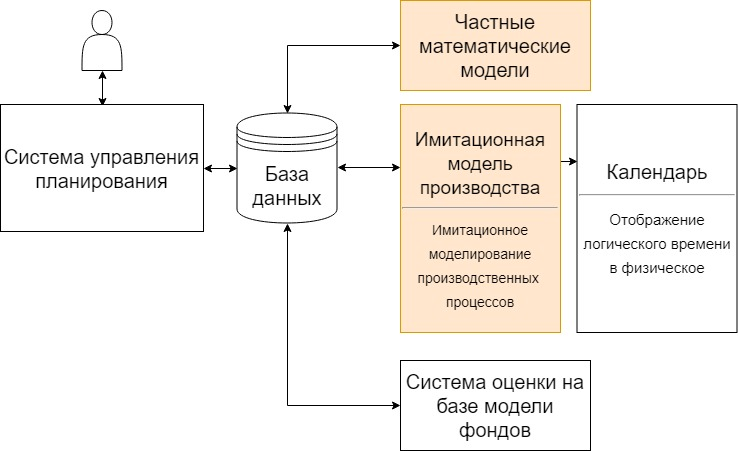
\includegraphics[width=1\linewidth]{fig/arh1.jpg}}
    \caption{Архитектура ПО}
    \label{ris:arh1}
\end{figure}

На рисунке \ref{ris:arh1} представлена архитектуры программного обеспечения. Данная архитектура содержит следующие элементы:

\begin{itemize}
    \item пользовательский интерфейс для взаимодействия с системой, который также позволяет получать информацию о работе системы в виде диаграмм, или графиков; 
    \item система управления планирования взаимодействует со всеми элементами системы и является главным распорядителем задач;
    \item база данных хранит всю информацию о производстве и результаты планирования; 
    \item имитационная модель производства создает план на основе информации из технологической карты и производственного плана;
    \item календарь обрабатывает абсолютные значения, используемые при планировании, и привязывает их к конкретным датам;
    \item частные оптимизационные модели работают с уже сформировавшимся планом, который получен в результате имитационного моделирования. К данному плану применяются алгоритмы оптимизации, зависящие от конкретных целей. Таким целями могут быть: задачи упорядочивания, задачи согласования, задачи распределения, задачи с суммарными критериями оптимизации, задачи с минимаксимальными критериями оптимизации[1, 2].
\end{itemize}

\section{Архитектура имитацонной модели}

\section{Частные оптимизационные модели}

\section{Выбор технологии реализации}

Про golang